\documentclass[a4paper]{scrartcl}
\usepackage[a4paper,top=2cm,bottom=2cm,left=2cm,right=2cm]{geometry}
\usepackage[utf8x]{inputenc}
\usepackage{graphicx}
\usepackage[T1]{fontenc}
\usepackage[italian]{babel}
\usepackage{tabularx}
\usepackage{helvet}
\usepackage{longtable}
\usepackage{booktabs}
\usepackage{xcolor}
\usepackage{amsfonts}
\usepackage{listings}

\renewcommand{\familydefault}{\sfdefault}

\definecolor{keyword}{RGB}{155,0,20}

% Informazioni generali
\newcommand{\corso}{Basi di Dati}
\newcommand{\anac}{A.A. 2014/2015}
\newcommand{\laurea}{Corso di Laurea Magistrale in Ingegneria Informatica}
\newcommand{\matricola}{1110975}
\newcommand{\nome}{Luca}
\newcommand{\cognome}{Vallerini}
\newcommand{\data}{Data di consegna: 15 giugno 2015}
\newcommand{\consegna}{Homework 4 - Progettazione Fisica}

\begin{document}

% Intestazione con loghi
\begin{figure}
	\begin{minipage}[t]{\textwidth}
		
\includegraphics[height=15mm]{img/logounipd}
		\hfill
		
\includegraphics[height=15mm]{img/logodei}
	\end{minipage}
\end{figure}

% Intestazione corso
{
\centering
\textbf{\corso , \anac} \\
\textbf{\laurea} \\
\vspace{5pt}
\textbf{\consegna} \\
\textbf{\small\data}


% Intestazione dati studente
\begin{table}[h]
	\begin{tabularx}{\textwidth}{|X|X|X|}
		\hline
		\multicolumn{1}{|c|}{\textbf{Cognome}} &
		\multicolumn{1}{c|}{\textbf{Nome}} &
		\multicolumn{1}{c|}{\textbf{Numero di matricola}} \\
		\centering\cognome &
		\centering\nome &
		\centering\matricola \tabularnewline
		\hline
	\end{tabularx}
\end{table}

}	

% Svolgimento
\subsection*{\color[RGB]{155,0,20}Schema fisico}
\lstinputlisting[language=SQL, basicstyle=\tiny , breaklines=true, commentstyle=\color{gray}, keywordstyle=\color{keyword}, numbers=left, tabsize=2,
otherkeywords={REFERENCES, ENUM, TYPE, boolean, money, bytea, text}, numberstyle=\tiny\color{gray}]{code/schemaFisico.sql}

\subsection*{\color[RGB]{155,0,20}Esempio di popolamento della base di dati}
\lstinputlisting[language=Java, basicstyle=\tiny , breaklines=true, commentstyle=\color{gray}, keywordstyle=\color{keyword}, numbers=left, tabsize=2, numberstyle=\tiny\color{gray}]{code/InsertDataFumetteria.java}

\subsection*{\color[RGB]{155,0,20}Interrogazioni principali}
\lstinputlisting[language=SQL, basicstyle=\tiny , breaklines=true, commentstyle=\color{gray}, keywordstyle=\color{keyword}, numbers=left, tabsize=2,
otherkeywords={REFERENCES, ENUM, TYPE, boolean, money, bytea, text}, numberstyle=\tiny\color{gray}]{code/QueryPrincipali.sql}

\subsection*{\color[RGB]{155,0,20}Implementazione JDBC delle interrogazioni principali e visualizzazione}
\lstinputlisting[language=Java, basicstyle=\tiny , breaklines=true, commentstyle=\color{gray}, keywordstyle=\color{keyword}, numbers=left, tabsize=2, numberstyle=\tiny\color{gray}]{code/QueryPrincipali.java}

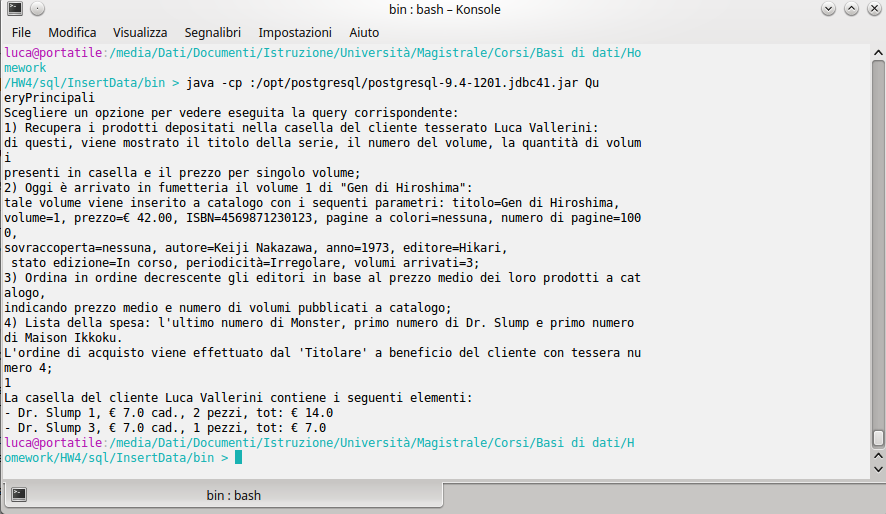
\includegraphics[width=\linewidth]{img/query1_1}
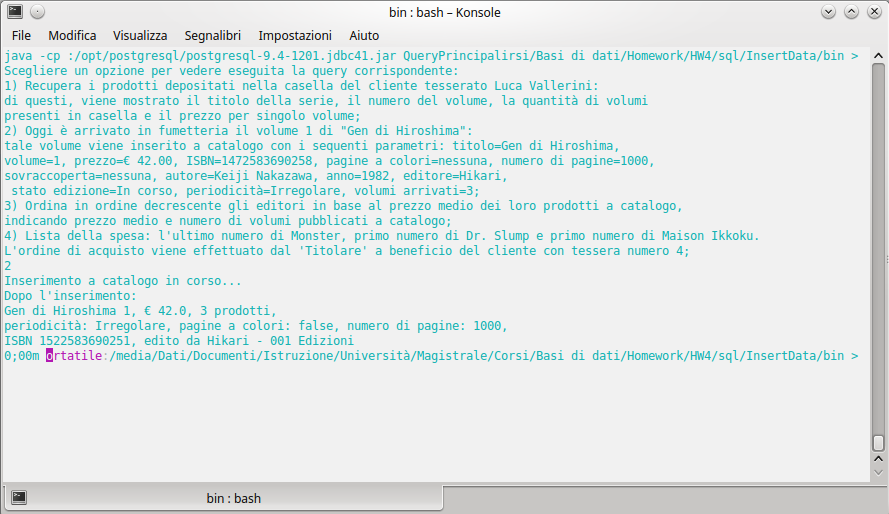
\includegraphics[width=\linewidth]{img/query2_1}
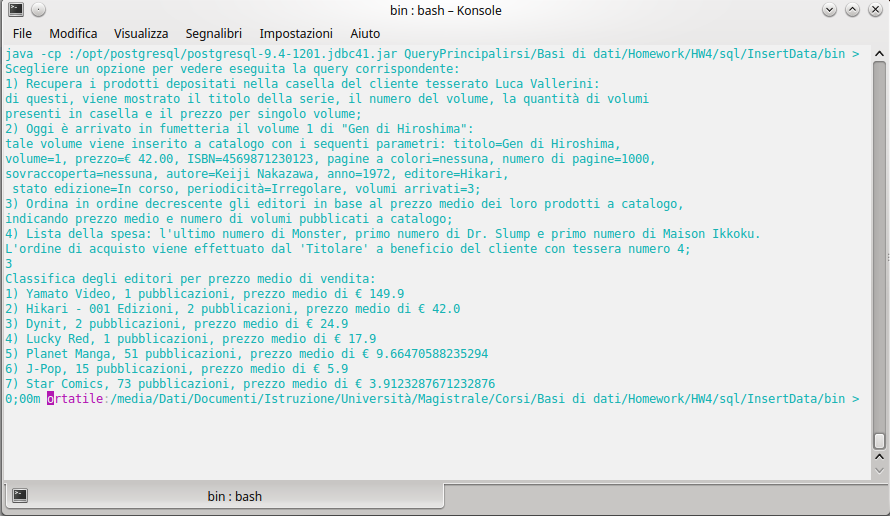
\includegraphics[width=\linewidth]{img/query3_1}
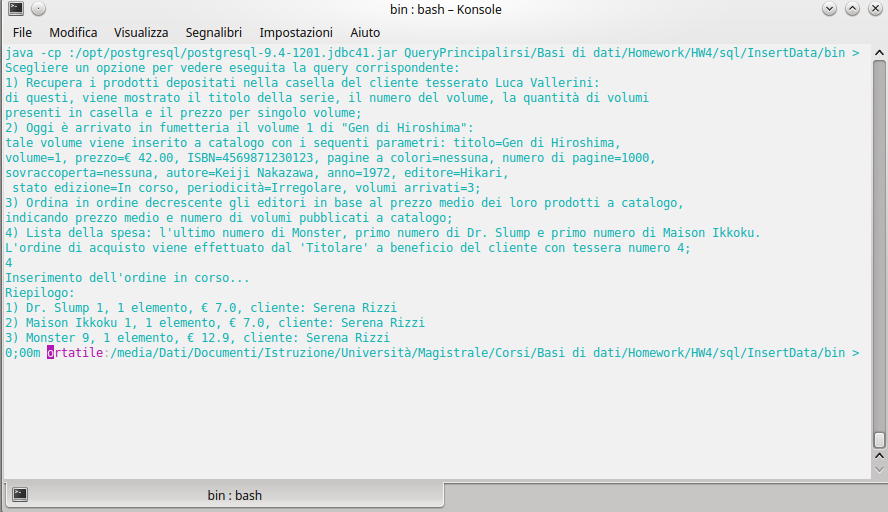
\includegraphics[width=\linewidth]{img/query4_1}

\end{document}